\chapter{Machine Learning and/or Analytical Models to Predict GPU Applications}

% \section{Introduction} 
% \label{sec:Intro}
Today, most computing platforms for HPC have heterogeneous hardware resources (CPUs, GPUs, storage, etc.). The most powerful supercomputers today have millions of those resources. In order to use all the computational power available, applications must be composed of multiple tasks that must use all available resources as efficiently as possible.
 
The Job Management System (JMS) is the middleware responsible for distributing computing power to applications. The JMS requires that users provide an upper bound of the execution times of their jobs (wall time). Usually, if the execution goes beyond this upper bound, the job is killed. This leads to very bad estimations, with an obvious bias that tends to overestimate their durations~\cite{Gaj:Trystram:2002}.

Graphics Processing Units (GPUs) are specialized processing units that were initially conceived with the purpose of accelerating vector operations, such as graphics rendering. GPUs are general purpose parallel processing units with accessible programming interfaces, including standard languages such as C, Java and Python. In particular, the Compute Unified Device Architecture (CUDA) is a parallel computing platform that facilitates the development on any GPU manufactured by NVIDIA~\cite{CUDAGuide}. CUDA was introduced by NVIDIA in 2006 for their GPU hardware line.

Information from profiling and traces of heterogeneous applications can be used to improve current JMSs, which require a better knowledge about the applications~\cite{ Gaussier:2015}.
Predicting execution times in heterogeneous applications is a great challenge, because hardware characteristics can impact their performance in different ways. Some parallel programs can be efficiently executed on some architectures, but not on others. 

Parallel computing models have been an active research topic since the development of modern computers~\cite{Juurlink:1998}. Preliminary works on the characterization of the performance of GPU applications on heterogeneous platforms showed that simple analytical models can be used to predict performance of such applications~\cite{BSPGPUCache:2015,PredicModelGPU2009} 

In this paper, we implemented a fair comparison between different machine learning approaches and a simple BSP-based model to predict the execution time of GPU applications~\cite{BSPGPUCache:2015}. The experiments were made using 9 different applications that perform vector operations. We used 9 different NVIDIA GPUs in the experiments, 6 from Kepler and 3 from Maxwell architecture. 

Our main contribution was showing that machine learning techniques provided acceptable predictions for all the applications over all the GPUs. Although the analytical model provided better predictions, it requires knowledge on the application and hardware structure. Consequently, machine learning techniques can be useful for deploying automated on-line performance prediction for scheduling applications on heterogeneous architectures with GPUs, whenever a large data set with information about similar applications is available.

The rest of this paper is organized as follows: In Section~\ref{sec:Background}, we present important concepts to understand this work. In Section~\ref{sec:RelatedWork}, we review the literature about the area. In Section~\ref{sec:Metho}, we describe our experiments and methodology. In Section~\ref{sec:Results}, we present the results from the experiments. Finally, in Section \ref{sec:Conclusions}, we present the conclusions of our work and future work.


% \section{Background}\label{sec:Background}
% 
% \subsection{NVIDIA GPU Microarchitecture and CUDA} \label{ssec:GPUs}

NVIDIA GPU architectures have multiple asynchronous parallel Streaming Multiprocessors (SMs) which contain Scalar Processors (SPs), Special Function Units (SFUs) and load/store units. These GPU architectures vary on a large number of features, such as number of cores, registers, SFUs, load/store units, on-chip and cache memory sizes, processor clock frequency, memory bandwidth, unified memory spaces and dynamic kernel launches. Those differences are summarized in the Compute Capability (C.C.) of an GPU.

The main advantage of GPUs is that they contains thousands of simple cores, which can be used concurrently by many threads. NVIDIA GPUs have hierarchical memory configuration with a global memory, which is shared among all threads. Concurrent accesses by threads from the same warp (groups of 32 threads) to contiguous addresses can be coalesced in a single transaction. But it has a latency of about 400 or 600 cycles per access \cite{GPU:BenchMark}. To improve memory access efficiency, they provide a small on-chip shared memory, which has a low-latency and can be accessed by all threads in a single SM. Fermi and Kepler also provide a low-latency on-chip L1 cache, with a small access latency. A L2 off-chip cache is also present, with a latency higher than L1 cache, but lower than the global memory. %Figure \ref{fig:hierarchyThread} shows the hierarchy memory accessed by any thread executed in a Kepler and Maxwell architecture.

% \begin{figure}[htpb]
%  \centering
%  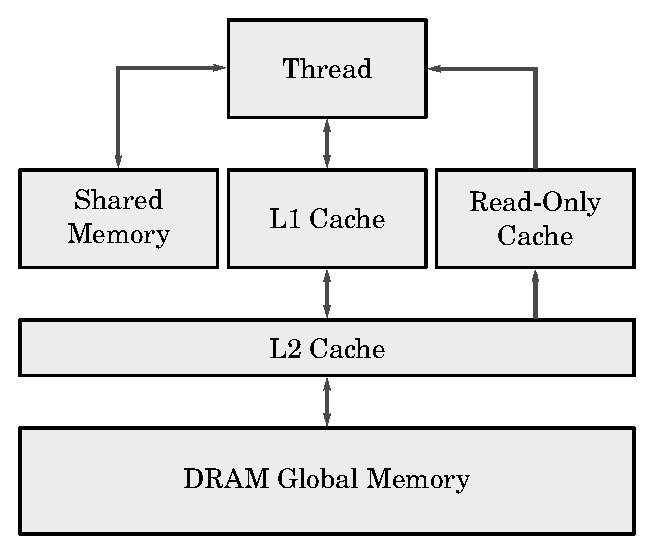
\includegraphics[scale=.5]{./images/GPUthreads.eps}
%  \caption{Memory hierarchy for threads from a kernel executed in Kepler architectures}
%  \label{fig:hierarchyThread}
% \end{figure}

The CUDA programming model and platform enables the use of NVIDIA GPUs for scientific and general purpose computations. A single \textit{master} thread runs in the CPU, launching and managing computations on the GPU. 
Data for the computations has to be transferred from the main memory to the GPU's memory.

\subsection{Bulk Synchronous Parallel Model}\label{ssec:AnalyticalModel}
The main goal of parallel computing models is to provide a standard way of describing and evaluating the performance of parallel applications. For a parallel computing model to succeed, it is paramount to consider the characteristics of the underlying architecture of the hardware used.

One of the most well-established models for parallel computing is the
Bulk Synchronous Parallel (BSP), first introduced by Valiant in
1990~\cite{Valiant:1990}. The computations in BSP model are organized in a sequence of \emph{supersteps}, each one divided into three successive---logically disjointed---phases. On the first phase, all processors use their local data to
perform local sequential computations in parallel (i.e., there is no communication among the processors.) The second phase is a communication phase, where all nodes exchange data performing personalized all-to-all
communication. The last phase consists of a global synchronization
barrier, that guarantees that all messages were delivered and all
processors are ready to start the next superstep. 
% Figure~\ref{fig:BSP} depicts the phases of a BSP application. 

% \begin{figure}[htpb]
% \centering
% \includegraphics[scale=.4]{./images/bspmodel.eps}
% \caption{Superstep in a Bulk Synchronous Parallel Model.}
% \label{fig:BSP}
% \end{figure}

The cost to execute the $i$-th superstep is then given by:
\begin{equation}
  \label{eq:superstep-cost}
  w_i + g h_i + L
\end{equation}

where $w_i$ is the maximum amount of local computations executed, and $h_i$ is the largest number of packets sent or received by any processor during the superstep. If $W = \sum_{i=1}^{S} w_i$ is the sum of the maximum work executed on all supersteps and $H = \sum_{i=1}^{S} h_i$ the sum of the maximum number of messages exchanged in each superstep, then the total execution time of the application is given by:
\begin{equation}
  \label{ec:BSP}
  T = W + g H + L S
\end{equation}
It is common to present the parameters of the BSP model as a tuple $(w,g,h,L)$.

\subsection{BSP-based Model for GPU Applications}\label{ssec:GPUModel}
In \cite{BSPGPUCache:2015} the authors created a simple BSP-based model to predict performance in GPU applications. This model abstracts all the heterogeneity of GPU architectures and many optimizations that GPU application can perform in a parameter $\lambda$. We have used this model to do the comparison with the machine learning approaches. The equation \ref{ec:BSPGPU} shows the predicted running time of a kernel $T_k$ using this model.

\begin{equation}\label{ec:BSPGPU}
T_k = \frac{t \cdot (Comp + Comm_{GM} + Comm_{SM})}{R \cdot P \cdot \lambda}
\end{equation} 

 \noindent $t$ is the number of threads launched, $Comp$ is the computational cost of one thread, number of cycles spent by each thread in computations, $Comm_{GM}$ is the communication cost of global memory accesses of one thread (Equation~\ref{ec:GM}), $Comm_{SM}$ is the communication cost of shared memory accesses of one thread (Equation~\ref{ec:SM}), $R$ is the clock rate, $P$ is the number of cores, $\lambda$ models the effects of application optimizations.

\begin{equation}\label{ec:SM}
Comm_{SM} = \left(ld_{0} + st_{0} \right) \cdot g_{SM}
\end{equation}


\begin{equation}\label{ec:GM}
Comm_{GM} = \left(ld_{1} + st_{1} - L1 - L2 \right) \cdot g_{GM} +  L1\cdot g_{L1} + L2\cdot g_{L2} 
\end{equation}

\noindent where $g_{SM}$, $g_{GM}$, $g_{L1}$ and $g_{L2}$ are constants representing the latency in communication over shared, global, L1 cache and L2 cache memory, respectively. $ld_0$ and $st_0$ represent the average number of load and stores for one thread in the shared memory, and $ld_1$ and $st_1$ global memory. $L1$ and $L2$ are average cache hits in $L1$ and $L2$ cache for one thread. $L1$ caching in Kepler and Maxwell architectures is reserved for register spills in local memory. For this reason $L1$ is always 0 for all the experiments. Global loads are cached in $L2$ only.

The parameter $\lambda$ captures the effects of thread divergence, global memory access optimizations, and shared memory bank conflicts. t is used to adjust the predicted application execution time with the measured one and is defined as the ratio between these values. It needs to be measures only once, for a single input size and a single board. The same lambda should work for all input sizes and boards of the same architecture. For a better description of this analytical model, more info can be found in \cite{BSPGPUCache:2015}.

Intra-block synchronization is very fast, and did not need to be included. Nevertheless, we maintained the inspiration on the BSP-model because the extended version of the model for multiple GPUs needs global synchronizations.

\subsection{Machine Learning}\label{ssec:ML}
Machine learning refers to a set of techniques for understanding data. The theoretical subject of ``learning'' is related to prediction. Machine learning techniques involve building a statistical model for predicting, or estimating an output based on one or more inputs. Regression models are used when the output is a continuous value. In this paper, we used three different machine learning methods: Linear Regression, Support Vector Machines and Random Forest. There exists other machine learning techniques with sophisticated learning process. However, in this work, we wanted to use simple models to prove that they achieve reasonable predictions.

\subsubsection{\textbf{Linear Regression (LR)}}
Linear regression is a straightforward technique for predicting a quantitative response $Y$ on the basis of a single or multiple predictor variables $X_p$. It assumes that there is approximately a linear relationship between each $X_p$ and $Y$. It gives to each predictor a separate slope coefficient in a single model. Mathematically, we can write the multiple linear regression model as
\begin{equation}
Y \approx \beta_0 + \beta_1 X_1 + + \beta_2 X_2 + \ldots + + \beta_p X_p + \epsilon
\end{equation}
where $X_p$ represents the $p$th predictor and $\beta_p$ quantifies the association between that variable and the response.

\subsubsection{\textbf{Support Vector Machines (SVM)}}
Support Vector Machines is a widely used technique for classification and regression problems. It belongs to the general category of kernel methods, which are algorithms that depend on the data only through dot-products. The dot product can be replaced by a kernel function which computes a dot product in some possibly high dimensional feature space $Z$. It maps the input vector $x$ into the feature space $Z$ though some nonlinear mapping. 

\subsubsection{\textbf{Random Forest (RF)}} 
Random Forests belong to decision tree methods, capable of performing both regression and classification tasks. In general, a decision tree with $M$ leaves divides the feature space into $M$ regions $R_m$, $1 \leq m \leq M$. The prediction function of a tree is then defined as $f(x) = \sum_{m=1}^{M} c_m I(x, R_m)$, where $M$ is the number of leaves in the tree, $R_m$ is a region in the features space, $c_m$ is a constant corresponding to region $m$ and $I$ is the indicator function, which is 1 if $x \in R_m$, 0 otherwise. The values of $c_m$ are determined in the training process. Random forest consists of an ensemble of decision trees and uses the mode of the decisions of individual trees.


\section{Related Work}\label{sec:RelatedWork}
Juurlink et al. were one of the firsts authors to compare performance predictions of parallel computing models~\cite{Juurlink:1998}, comparing BSP, E-BSP and BPRAM over different parallel platform. Some authors have also focused their work in performance prediction of parallel applications using machine learning~\cite{Singh:2007:PPA}. All this work is about parallel applications executed over CPUs and not GPU applications.

In  recent  years,  studies on GPU performance using different statistical and machine learning approaches have appeared. Baldini et al. showed that machine learning can predict GPU speedup from OpenMP applications~\cite{Baldini:2014}. They used K-nearest neighbor and SVM as classifier to know the performance of these applications over different GPUs. Wu et al. described a GPU performance and power estimation model~\cite{Greathouse:2015:GPGPUML}, using K-means to create sets of scaling behaviors representative of the training kernels and neural networks that map kernels to clusters, with experiments using OpenCL applications over AMD GPUs. Karami et al. proposed a statistical performance prediction model for OpenCL kernels on NVIDIA GPUs~\cite{Karami:2013} using a regression model for prediction and principle component analysis for extracting features of higher weights, thus reducing model complexity while preserving accuracy. Zhang et al. presented  a statistical approach on  the  performance and power consumption of an ATI GPU~\cite{Zhang:2011}, using Random Forest due to its useful interpretation tools. Hayashi et al. constructed a prediction model that estimates the execution time of parallel applications~\cite{Hayashi:2015:MPH} based on a binary prediction model with Support Vector Machines for runtime CPU/GPU selection. Kerr et al. developed Eiger~\cite{Kerr:2012:Eiger}, which is a framework for automated  statistical approaches for modeling program behaviors on diverse GPU architectures. They used various approaches, among them principal component analysis, clustering techniques, and regression analysis. Madougou et al. presented a comparison between different GPGPU performance modeling tools~\cite{Madougou201618}, they compare between analytical model, statistical approaches, quantitative methods and compiler-based methods. Meswani et al. predicted the performance of HPC applications on hardware accelerators such as FPGA and GPU from applications running on CPU~\cite{6270861}. This was done by identifying common compute patterns or idioms, then developing a framework to model the predicted speedup when the application is run on GPU or FPGA using these idioms. Ipek et al. trained multilayer neural networks to predict different performance aspects of parallel applications using input data from executing applications multiple times on the target platform~\cite{Ipek:2005:APP:2138773.2138800}.

In this work, we compare three different machine learning techniques to predict kernel execution times over NVIDIA GPUs. We also perform a comparison with a BSP-based analytical model to verify when each approach is advantageous. Although some works have compared analytical models, statistical approaches and quantitative methods, to the best of our knowledge this is the first work that compares analytical model to machine learning techniques to predict running times of GPU applications. Moreover, it offers a comparison between different machine learning techniques.

\section{Methodology}\label{sec:Metho}
In this section we discuss the algorithms and GPU testbed, the analytical model and the methodology used in the learning process. During our evaluation, all applications were executed using the CUDA profiling tool \textit{nvprof}. Each experiment is presented as the average of ten executions, with a confidence interval of 95\%.

\subsection{Algorithm Testbed}\label{ssec:AlgTestbed}
The benchmark contains 4 different strategies for \emph{matrix multiplication}~\cite{CUDAGuide}, 2 algorithms for \emph{matrix addition}, 1 dot product algorithm, 1 vector addition algorithm and 1 \emph{maximum sub-array problem} algorithm~\cite{Cleber:Thesis}.

\subsubsection{\textbf{Matrix Multiplication}}
We used four different memory access optimizations: global memory with non-coalesced accesses (MMGU); global memory with coalesced accesses (MMGC); shared memory with non-coalesced accesses to global memory (MMSU); and shared memory with coalesced accesses to global memory (MMSC). The run-time complexity for a sequential matrix multiplication algorithm using two 
matrices of size $N\times{}N$ is $O(N^3)$. In a CUDA application with $N^2$ threads, the run-time complexity is $O(N)$ 

\subsubsection{\textbf{Matrix Addition}}
We used two different memory access optimizations: global memory with non-coalesced accesses (MAU); and global memory with coalesced accesses (MAC);  The run-time complexity for a sequential matrix addition algorithm using two 
matrices of size $N\times{}N$ is $O(N^2)$. In a CUDA application with $N^2$ threads, the run-time complexity is $O(1)$.

\subsubsection{\textbf{Vector Addition Algorithm (vAdd)}}
For two vectors $A$ and $B$, the Vector Addition $C = A + B$ is obtained by adding the corresponding components. In a GPU algorithm, each thread performs an addition of a position of the vectors $A$ and $B$ and stores the result in the vector $C$. 

\subsubsection{\textbf{Dot Product Algorithm (dotP)}}
For two vectors $A$ and $B$, the dot product $C = A \cdot B$ is obtained by adding the multiplication of corresponding components of the input, the result of this operation is a scalar. In a GPU algorithm, each thread performs a multiplication of a position of the vectors $A$ and $B$ and stores the result shared variable. Then a reduction per blocks is performed and a vector of size equal to the number of block in the grid is transferred to the CPU memory for later processing. 


\subsubsection{\textbf{Maximum Sub-Array Problem (MSA)}}
Let $X$ be a sequence of $N$ integer numbers $(x_1, ... , x_N)$. The Maximum Sub-Array Problem (SSM) consists of finding the contiguous sub-array within $X$ which has the largest sum of elements. The implementation used in this paper creates a kernel with 4096 threads, divided in 32 blocks with 128 threads~\cite{Cleber:Thesis}. The $N$ elements are divided in intervals of $N/t$, and each block receives a portion of the array. The blocks use the shared memory for storing segments, which are read from the global memory using coalesced accesses. Each interval is reduced to a set of 5 integer variables, which are stored in vector of size $5 \times t$ in global memory. This vector is then transferred to the CPU memory for later processing. 

\subsection{GPU Testbed}\label{ssec:GPUTestbed}
We performed our comparisons over several different NVIDIA microarchitectures. We used 9 GPUs, described in Table~\ref{tab:GPUs}. GPUs with Compute Capability 3.X belong to Kepler architecture. GPUs with Compute Capability 5.X belong to Maxwell architecture. 

\begin{table}[htpb]
    \centering
    \caption{Hardware specifications of the GPUs in the testbed}
    \scalebox{0.75}{
    \begin{tabular}{lccccccc}
        \toprule
        \textbf{Model}&\textbf{C.C.}&\textbf{Memory}&\textbf{Bus}&\textbf{Bandwidth}&\textbf{L2}&\textbf{Cores/SM}&\textbf{Clock} \\ \bottomrule
        GTX-680&3.0&2 GB&256-bit&192.2 GB/s&0.5 M&1536/8&1058 Mhz \\ \midrule 
        Tesla-K40&3.5&12 GB&384-bit&276.5 GB/s&1.5 MB&2880/15&745 Mhz \\ \midrule
        Tesla-K20&3.5&4 GB&320-bit&200 GB/s&1 MB&2496/13&706 MHz\\ \midrule
        Titan Black&3.5&6 GB&384-bit&336 GB/s&1.5 MB&2880/15 &980 Mhz \\ \midrule
        Titan&3.5&6 GB&384-bit&288.4 GB/s&1.5 MB&2688/14&876 Mhz\\ \midrule
        Quadro K5200&3.5&8 GB&256-bit&192.2 Gb/s&1 MB&2304/12&771 Mhz \\ \midrule
        Titan X&5.2&12 GB&384-bit&336.5 GB/s&3 MB&3072/24&1076 Mhz \\ \midrule
        GTX-980&5.2&4 GB&256-bit&224.3 GB/s&2 MB&2048/16&1216 Mhz \\ \midrule
        GTX-970&5.2&4 GB&256-bit&224.3 GB/s&1.75 MB&1664/13&1279 Mhz\\ \midrule
    \end{tabular}}
    \label{tab:GPUs}
\end{table}


\subsection{Data sets}\label{ssec:DataSets}
For the analytical model, each application was executed with input sizes of power of two. For problems of one dimension, 10 samples were taken, from $2^{18}$ until $2^{27}$. For problems of two dimensions, 6 samples were taken, all of them were squares matrices, with number of lines from $2^{8}$ until $2^{13}$.

For the machine learning analysis, we first collected the performance profiles (metrics and events) for each kernel and GPU. To be fair with the analytical model, we then choose similar communication and computation parameters to use as data input for the machine learning algorithms. We performed the evaluation using cross-validation, that is, for each target GPU, we performed the training using the other 8 GPUs, testing the model in the target GPU.

To collect data for the machine learning algorithms, we executed the two-dimensional applications using three different size for the CUDA thread blocks, $8^2$, $16^2$ and $32^2$, and input sizes from $2^{8}$ to $2^{13}$. We took 32 samples per block size, resulting in 96 samples per GPU and a total of 864 samples. For the uni-dimensional problems we used input sizes from $2^{18}$ to $2^{27}$ and took 69 samples for each configuration, resulting in 207 samples per GPU and a total of 1863 samples. For sub-array maximum problem, 96 samples with the original configuration were taken, for a total of 864 samples. 

We also evaluate a scenario were we collected more examples of a single application. We executed the matrix multiplication with shared memory and coalesced accesses (MMSC) using 8 configurations: 16, 64, 144, 256, 400, 576, 784, and 1024 threads per blocks. This resulted in a total of approximately 256 samples for GPU, and more than 2000 samples.

For each sample, the metrics, events and trace information were collected in different phases, therefore avoiding the overhead over the measured execution time of the application. The features which we used to feed the Linear Regression, Support Vector Machines and Random Forest algorithms are described in the Table \ref{tab:predictors}.

\begin{table}[htpb]
    \centering
    \caption{Features used as input in the machine learning techniques}
    \scalebox{.825}{
        \begin{tabular}{c  c} 
        \toprule
        \textbf{Feature}&\textbf{Description} \\\midrule
        \texttt{num\_of\_cores} & \specialcell{Number of cores per GPU} \\ \midrule
        \texttt{max\_clock\_rate} & \specialcell{GPU Max Clock rate} \\\midrule
        \texttt{Bandwidth} & \specialcell{Theoretical Bandwidth} \\\midrule
        \texttt{Input Size} & \specialcell{Size of the problem} \\\midrule
        \texttt{totalLoadGM} & \specialcell{Load transaction in Global Memory} \\\midrule
        \texttt{totalStoreGM} & \specialcell{Store transaction in Global Memory} \\\midrule
        \texttt{TotalLoadSM} & \specialcell{Load transaction in Shared Memory} \\\midrule
        \texttt{TotalStoreSM} & \specialcell{Store transaction in Global Memory} \\\midrule
        \texttt{FLOPS SP} & \specialcell{Floating operation in Single Precision} \\\midrule
        \texttt{BlockSize} & \specialcell{Number of threads per blocks} \\\midrule
        \texttt{GridSize} & \specialcell{Number of blocks in the kernel} \\\midrule
        \texttt{No. threads} & \specialcell{Number of threads in the applications } \\\midrule
        % \texttt{Executed IPC} & \specialcell{Instructions executed per cycle} \\\midrule
        \texttt{Achieved Occupancy } & \specialcell{Ratio of the average active warps per active cycle to the maximum number of warps ed on a multiprocessor.} \\\midrule
        \end{tabular}}
    \label{tab:predictors} 
\end{table}

To generate the flags \texttt{totalLoadGM}, \texttt{totalStoreGM}, \texttt{TotalLoadSM} and \texttt{TotalStoreSM}, the number of requests was divided by the number of transactions per request for each operation.

We first transformed the data to a $log_2$ scale and, after performing the learning and predictions, we returned to the original scale using a $2^{pred}$ transformation~\cite{Barnes:2008:RAS}, reducing the non-linearity effects. Figure~\ref{fig:QQplot} shows the difference between the trained model without (left-hand side graph) and with (right-hand side graph) logarithmic scale. The linear regression resulted in poor fitting in the tails, resulting in poor predictions. This problem was solved with the log transformation.



\begin{figure}[htpb]
 \centering
 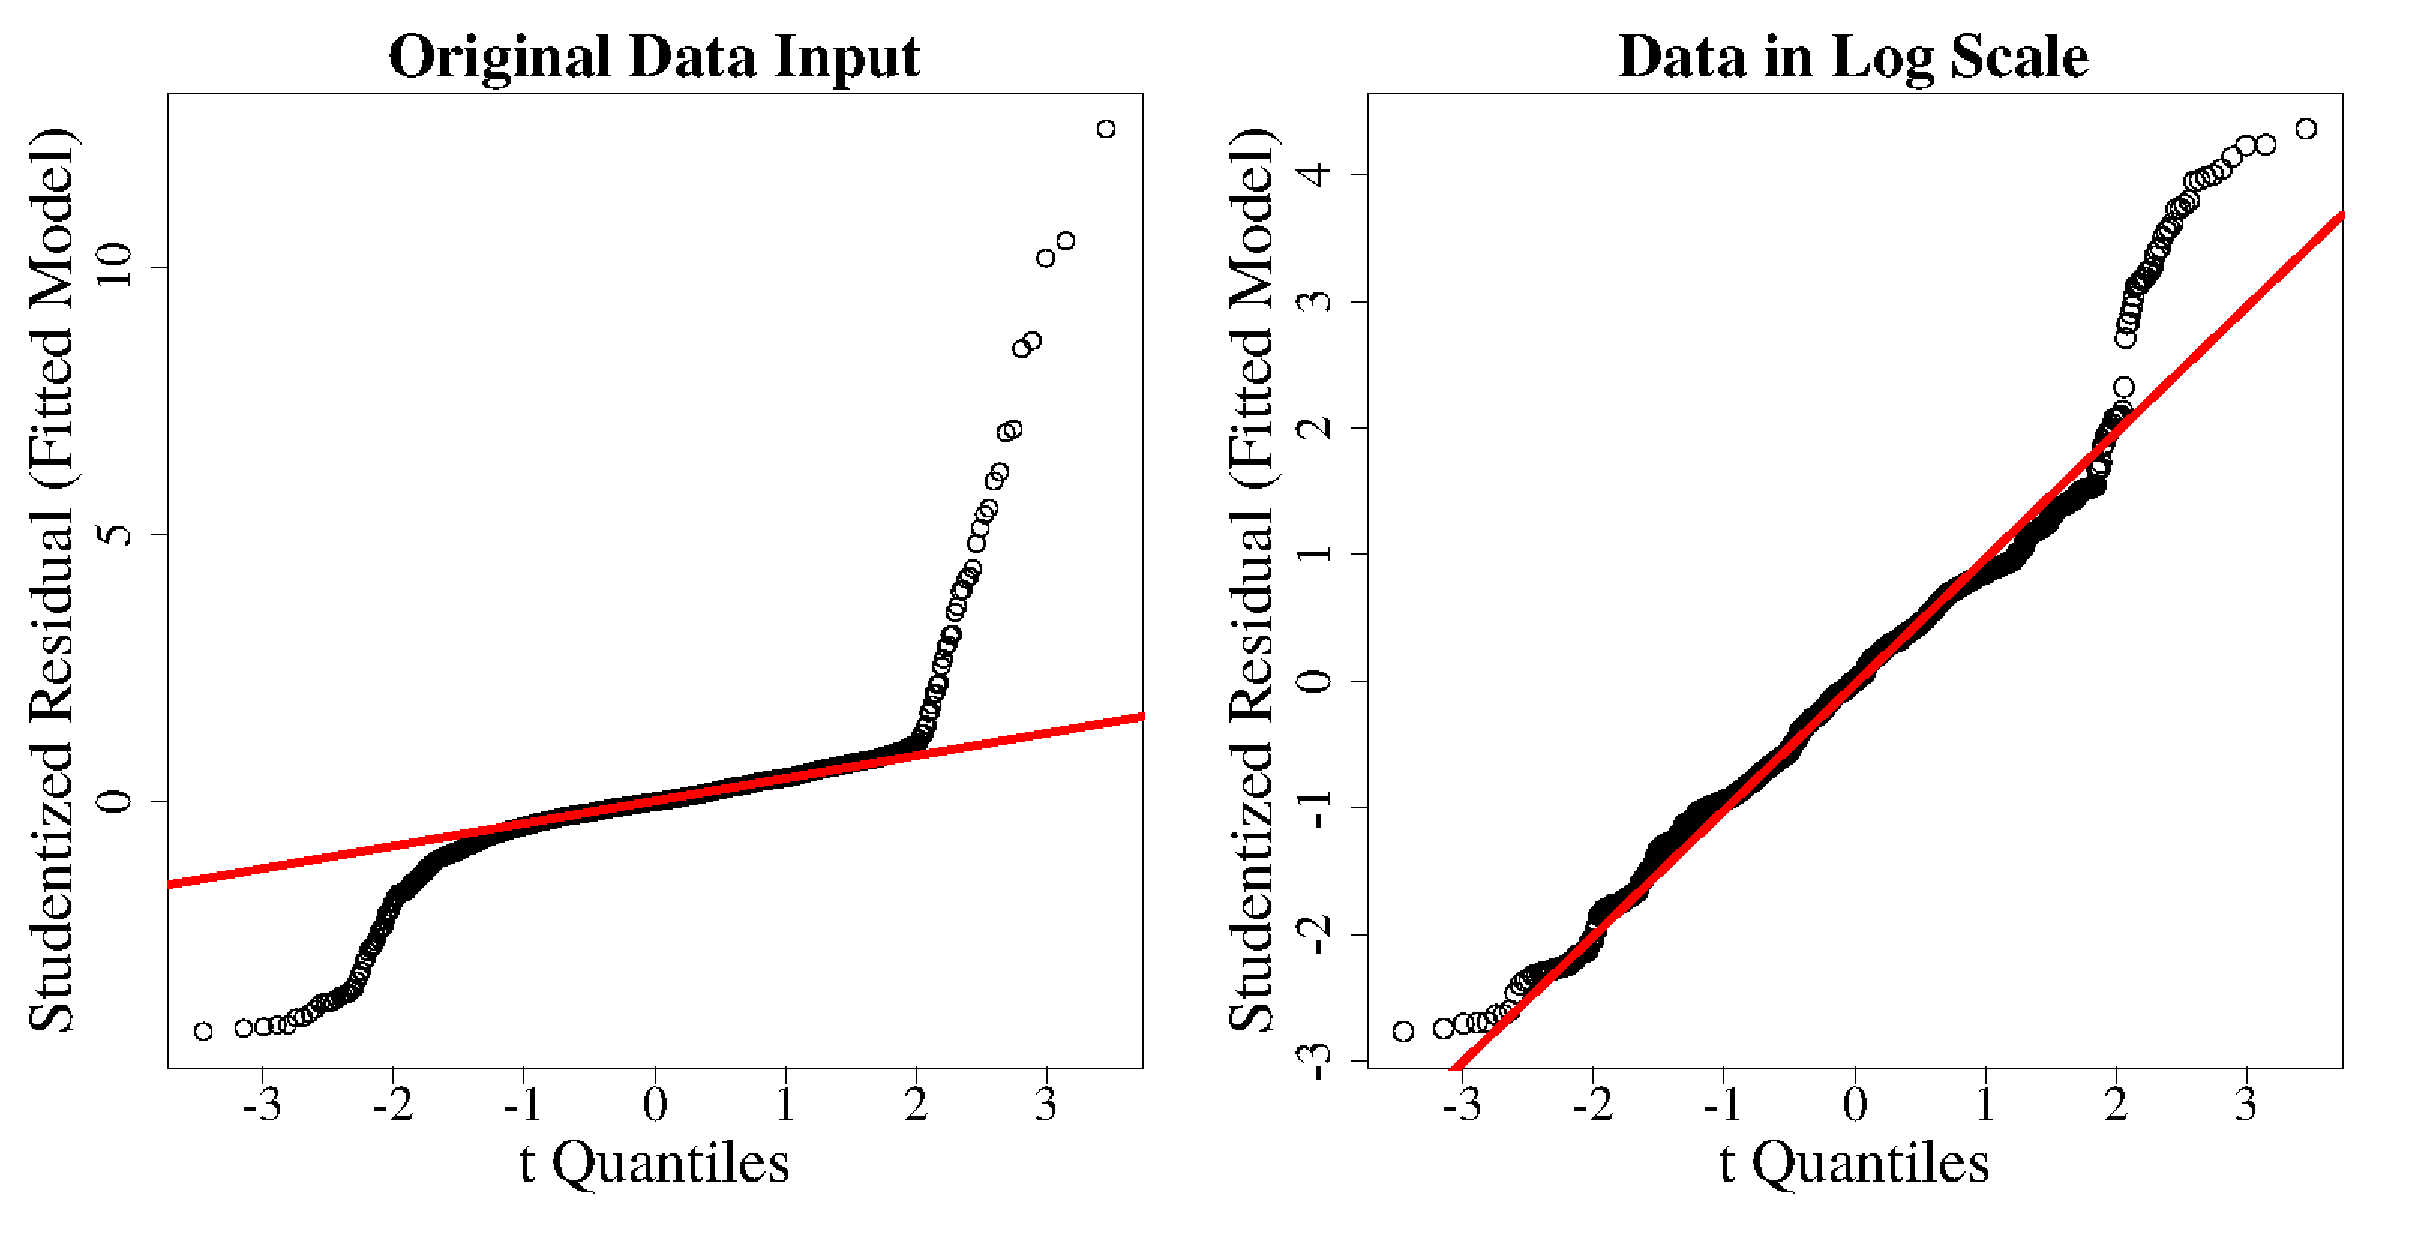
\includegraphics[scale=.2]{./images/QQplot.eps}
 \caption{Quantile-Quantile Analysis of the generated models}
 \label{fig:QQplot}
\end{figure}

In this work, we applied these methods over profiling information about metrics and events of the executions of GPU applications over NVIDIA GPUs. To measure the progress of the learning algorithm we have used the normalized mean square error. With this error we have analysed the reliability of our approaches.

We used R to automate the statistical analyses, in conjunction with the \texttt{e1071} and \texttt{randomForest} packages to use the \texttt{svm} and \texttt{randomForest} functions respectively.  

\section{Results}\label{sec:Results}

The  source code for all the experiments and results are
available\footnote{Hosted at GitHub: \texttt{\scriptsize https://github.com/marcosamaris/svm-gpuperf} [Accessed on 19 June 2016]} under Creative Commons Public License for the sake of reproducibility. The comparison between analytical models and machine learning approaches are done taking the accuracy of the predictions, defined as the ratio between the predicted and true values of execution times, i.e, $\frac{y_{pred}} { y_{true}}$.

The rest of this section is organized as follows: In subsection~\ref{subsec:Anamodel}, the Analytical model results are presented. In subsection~\ref{subsec:ML}, results for Machine Learning approach are presented. In subsection~\ref{subsec:both}, a comparison between the results of both approaches is presented.

\subsection{Analytical Model}\label{subsec:Anamodel}
The number of computation ($Comp$) and communication ($g_{SM}$, $g_{GM}$, $g_{L1}$ and $g_{L2}$) steps were extracted from the application source codes. These parameters are the same for all the simulations, and are presented in Table \ref{tab:AnaModel}. We did not include the values of the cache L2 for these experiments because they did not impact the execution times.

%{\huge VERIFICAR A TABELA}
\begin{table}[H]
\centering
\caption{Values of the model parameters over 9 different applications}
\scalebox{.65}{
\begin{tabular}{| c | c | c  |  c | c | c | c | c | c | c |} 
\midrule
\multirow{2}{*}{\textbf{Par.}} & \multicolumn{4}{c|}{\textbf{Matrix 
Multiplication}}&\multicolumn{2}{c|}{\textbf{Matrix 
Addition}}&\multirow{2}{*}{\textbf{vAdd}}&\multirow{2}{*}{\textbf{dotP}}&\multirow{2}{*}{\textbf{MSA}}
\\\cline{2-7}&\textbf{MMGU}&\textbf{MMGC}&\textbf{MMSU}&\textbf{MMSC}&\textbf{MAU}&\textbf{MAC}&&\\\midrule
$\mathbf{comp}$&\multicolumn{4}{c|}{$N\cdot$ FMA}&\multicolumn{3}{c|}{$1\cdot 24$}&$1\cdot 96$&$(N/t)\cdot 100 $\\\midrule
$\mathbf{ld_1}$&\multicolumn{4}{c|}{$2\cdot N$}&\multicolumn{3}{c|}{2}&2&$N/t$\\\midrule
$\mathbf{st_1}$&\multicolumn{4}{c|}{1}&\multicolumn{3}{c|}{2}&1&$N$\\\midrule
$\mathbf{ld_0}$&\multicolumn{2}{c|}{0}&\multicolumn{2}{c|}{$2\cdot N$}&\multicolumn{3}{c|}{0}
&0&$N/t$\\\midrule
$\mathbf{st_0}$&\multicolumn{2}{c|}{0}&\multicolumn{2}{c|}{1}&\multicolumn{3}{c|}{0}
&$1 + log(t)$&$5$\\
\midrule
\end{tabular}}
\label{tab:AnaModel} % is used to refer this table in the text
\end{table}

Different micro-benchmarks were used to measure the number of cycles per computation operation in GPUs~\cite{Bench:GPU}, with FMAs, additions and multiplications taking approximately 1, 24 and 96 cycles of clock. For all simulations, we considered $5$ cycles for latency in the communication for shared memory and $500$ cycles for global memory \cite{CUDAGuide}. Finally, when the models were complete, we executed a single instance of each application on each GPU to determine the $\lambda$ values, described in the Table \ref{tab:Lambda}.

\begin{table}[H]
\centering
\caption{Values of the parameter $\lambda$ for each application in each GPU}
\scalebox{0.6}{
\small
\begin{tabular}{| c | c | c  |  c | c | c | c| c | c | c |} 
\midrule%inserts double horizontal lines
&\textbf{MMGU}&\textbf{MMGC}&\textbf{MMSU}&\textbf{MMSC}&\textbf{MAU}&\textbf{MAC}&\textbf{dotP}&\textbf{vAdd}&\textbf{MSA}\\\midrule
GTX-680 & 4.25 & 19.00 & 18.00 & 68.00 & 0.85 & 11.00 & 14.00 & 11.00 & 0.68 \\ 
Tesla-K40 & 4.30 & 20.00 & 19.00 & 65.00 & 2.50 & 9.50 & 9.00 & 10.00 & 0.48 \\ 
  Tesla-K20 & 4.50 & 21.00 & 18.00 & 52.00 & 2.50 & 9.00 & 9.00 & 10.00 & 0.50 \\ 
  TitanBlack & 3.75 & 17.00 & 16.00 & 52.00 & 1.85 & 8.00 & 7.00 & 8.50 & 0.35 \\ 
  Titan & 4.25 & 21.00 & 17.00 & 50.00 & 2.50 & 10.00 & 9.50 & 12.00 & 0.48 \\
  Quadro & 5.00 & 22.00 & 22.00 & 68.00 & 1.25 & 10.00 & 12.00 & 11.00 & 0.50 \\ 
  TitanX & 9.00 & 38.00 & 38.00 & 118.00 & 2.75 & 10.50 & 7.50 & 10.50 & 1.05 \\ 
  GTX-980 & 9.00 & 40.00 & 40.00 & 110.00 & 3.25 & 9.75 & 10.00 & 10.00 & 1.65 \\ 
  GTX-970 & 5.50 & 26.00 & 24.00 & 75.00 & 1.85 & 5.90 & 7.00 & 6.00 & 1.05 \\\midrule
\end{tabular}
}
\label{tab:Lambda} 
\end{table}

\subsection{Machine Learning Approaches}\label{subsec:ML}

Figure~\ref{fig:AccMMSC} shows the box plots of the accuracy of the machine learning techniques using many samples. The box plots show the median for each GPU and the upper and lower first quartiles, with whiskers representing the 95\% confidence interval. Outliers are marked as individual points.

In this experiment, approximately 260 samples of the application MMSC were collected in each one of the 9 GPUs. For the training set 8 GPUs were used, and the remaining GPU was used for the test set. This was made for each GPU in the three techniques of machine learning. We can see that Linear Regression, Support Vector Machines and Random Forest have a reasonable accuracy for all the GPUs, with a mean between 0.75 and 1.5, for most cases, with some outliers.

The linear kernel in the support vector machine achieved the best performance and accuracy in the prediction. For this reason, Figures \ref{fig:AccMMSC}, \ref{fig:AccuracyAM} show similar results for Linear Regression and for Support Vector Machines. Other kernel like Polynomial, Gaussian (RBF) and Sigmoid were tested, they resulted in worse predictions. 

For the random forest, we have changed two default parameters, the number of trees and the number of variables as candidates at each split. For the first parameter, the default value was 500 and for the second parameter, the default value was $p/3$, where $p$ is the number of predictors, $13$ in this case according to Table \ref{tab:predictors}. We set the number of trees to $50$, and the number of predictors to split to $5$. These values achieved better prediction, and they were determined manually after many simulations.

\begin{figure}[htpb]
\centering
 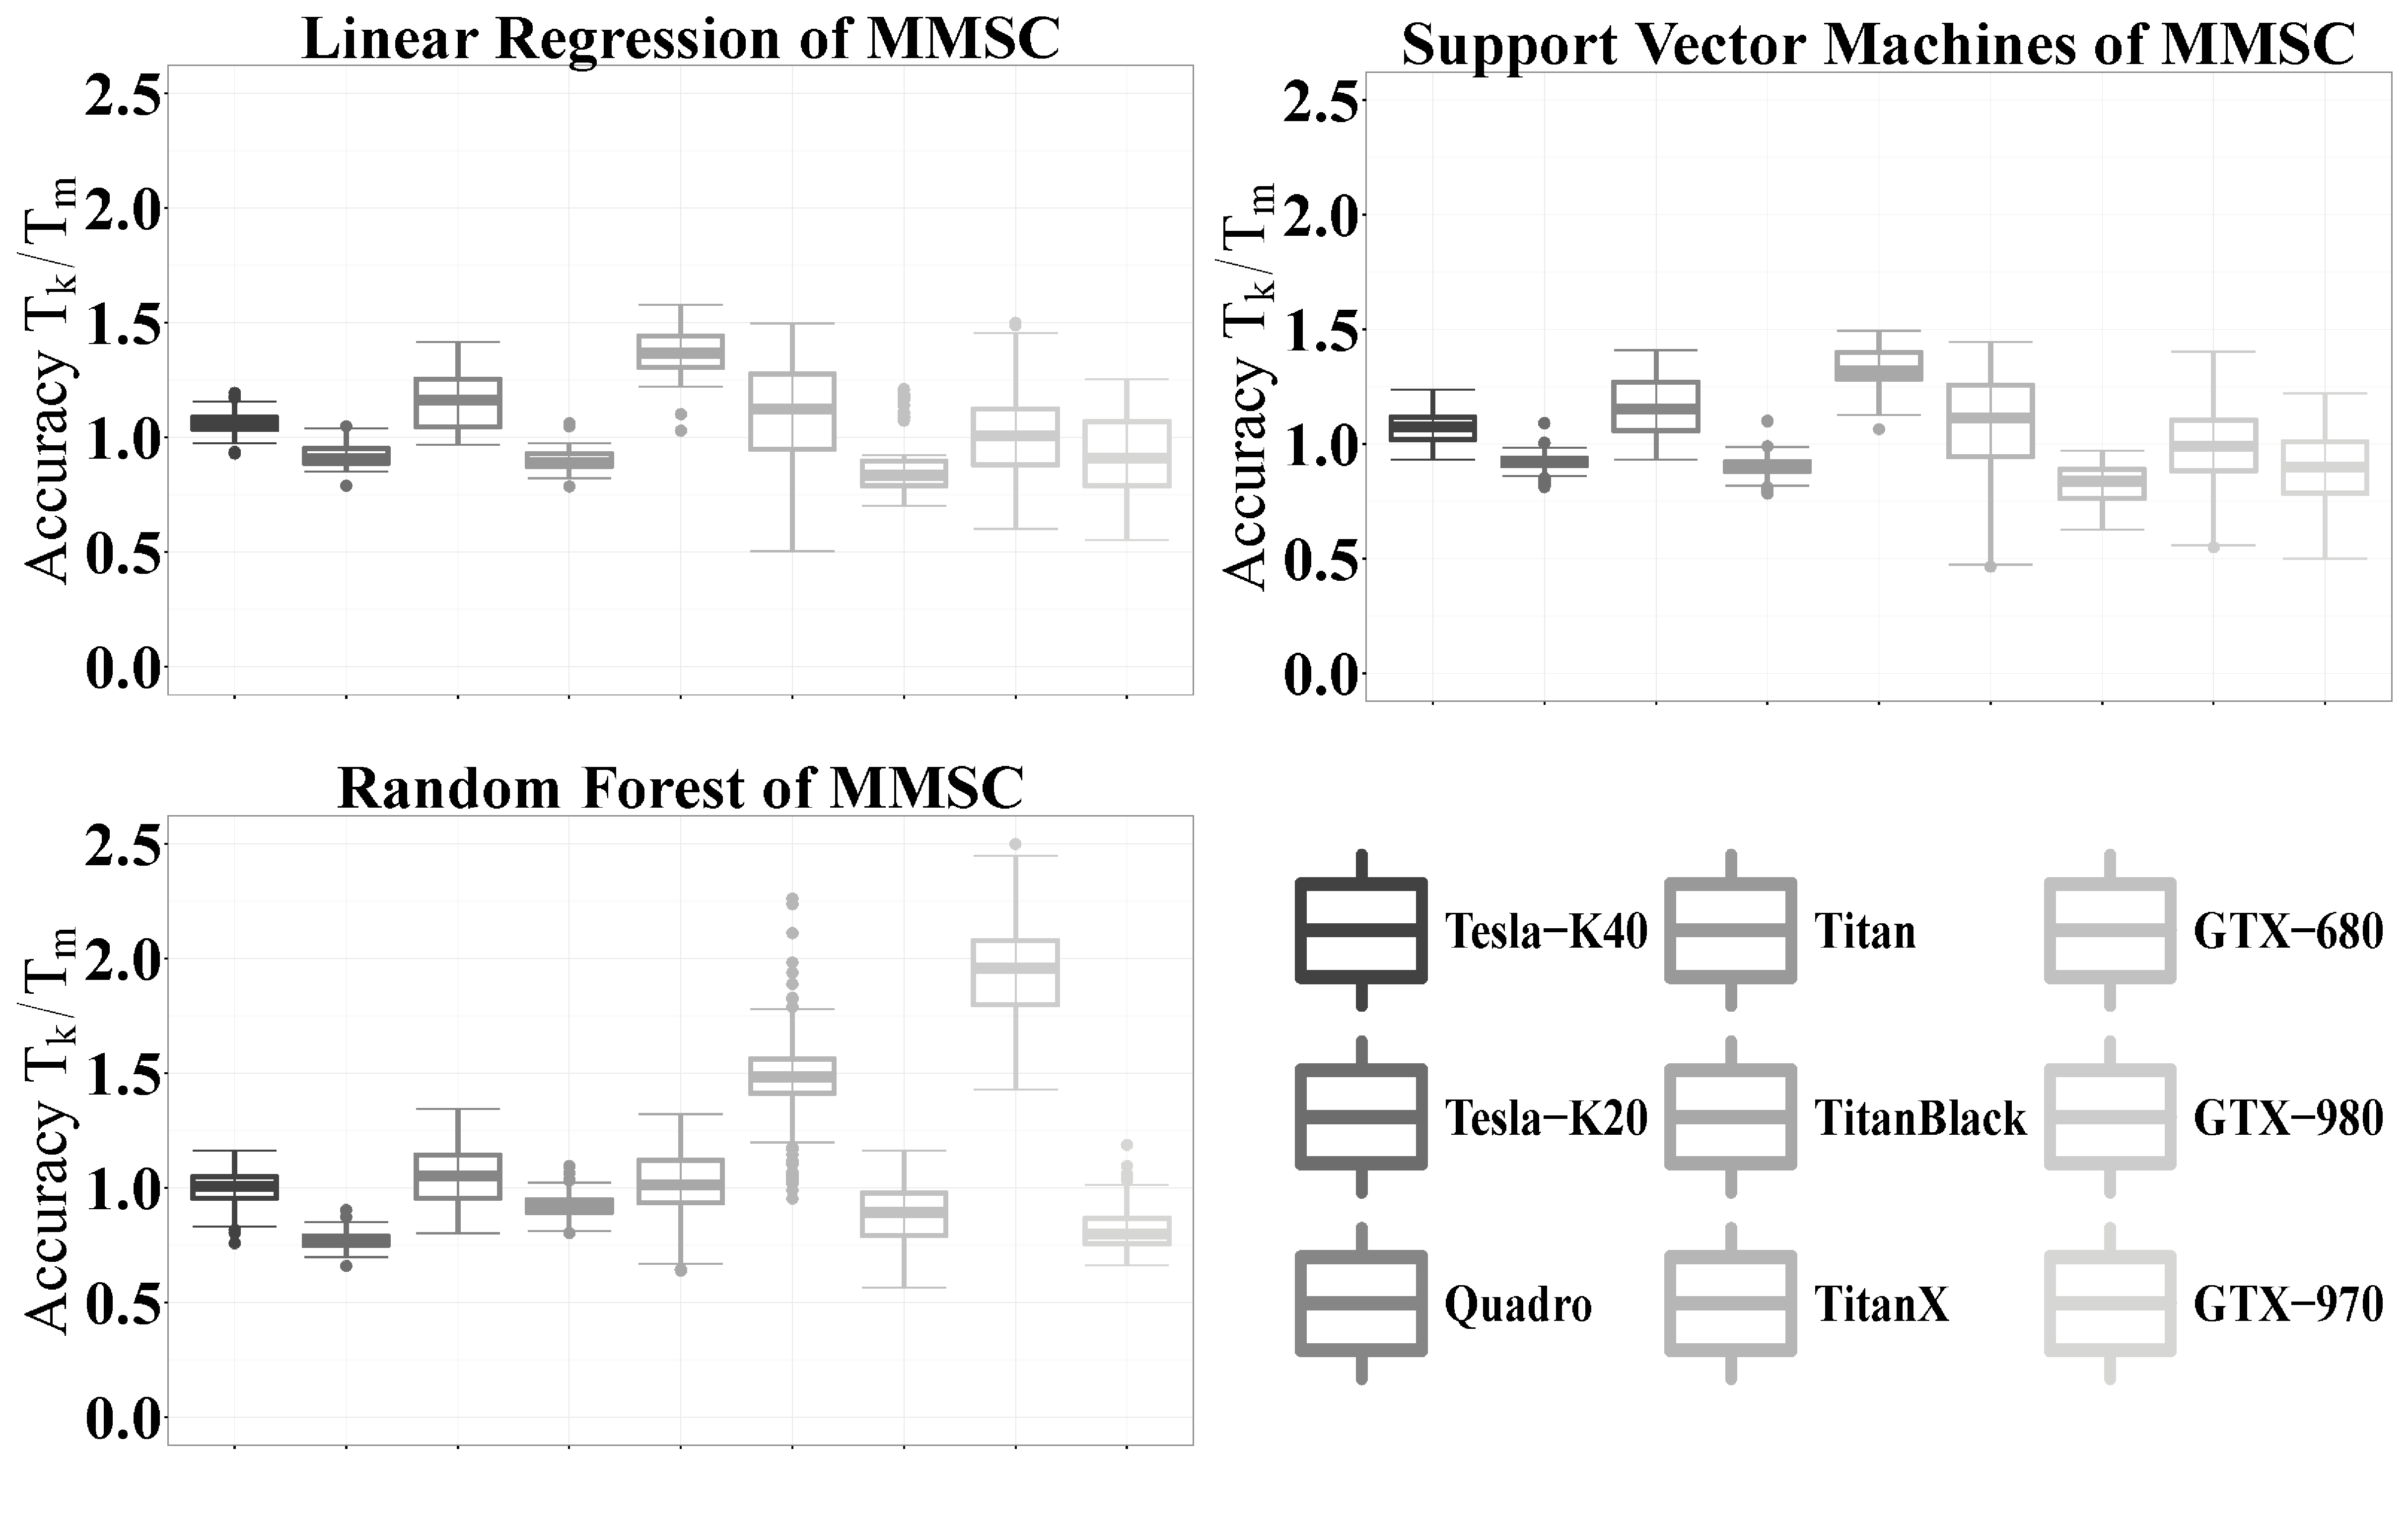
\includegraphics[scale=.11]{./images/MSCoalesced.eps}
  \caption{Accuracy of Machine Learning Algorithms of matMul-SM-Coalesced with many samples}
 \label{fig:AccMMSC}
\end{figure}

Table~\ref{tab:StatML} shows the comparison between the different regression models used, in terms of mean accuracy and mean squared error. In this table, we can see that the accuracy of the predictions are between 0.75 and 1.2 for almost all the cases, only the predictions of the GTX-980 with the Random Forest showed irregular predictions, we think that was because the application MMSC showed the best performance in this GPU and the selected parameters to split the decision tree lied at the moment of the predictions. 

\begin{table}[htpb]
\centering
\caption{Statistics of the Machine learning with more of 1000 samples for training process}
\scalebox{0.825}{
\small
\begin{tabular}{| c | c | c  |  c | c | c | c | c | c | c| c | c | } 
\midrule%inserts double horizontal lines
\multirow{2}{*}{\textbf{GPUs}}&\multicolumn{3}{c|}{\textbf{Accuracy Mean}}& \multicolumn{3}{c|}{\textbf{NMSE}}\\
    &\textbf{LR}&\textbf{SVM}&\textbf{RF}&\textbf{LR}&\textbf{SVM}&\textbf{RF}\\\midrule
GTX-680     &0.85 $\pm$ 0.09&0.82 $\pm$ 0.07&0.78 $\pm$ 0.08&0.033&0.037&\textbf{0.026}\\ 
Tesla-K40   &1.21 $\pm$ 0.05&1.20 $\pm$ 0.06&0.97 $\pm$ 0.06&0.006&0.008&\textbf{0.005}\\ 
Tesla-K20   &0.85 $\pm$ 0.03&0.84 $\pm$ 0.03&0.77 $\pm$ 0.02&\textbf{0.008}&\textbf{0.008}&0.051\\ 
Titan-Black &1.18 $\pm$ 0.07&1.16 $\pm$ 0.06&1.12 $\pm$ 0.12&\textbf{0.145}&0.115&0.019\\ 
Titan       &0.96 $\pm$ 0.04&0.96 $\pm$ 0.04&0.98 $\pm$ 0.06&0.012&0.012&\textbf{0.008}\\ 
Quadro      &1.00 $\pm$ 0.10&1.01 $\pm$ 0.10&0.98 $\pm$ 0.10&0.041&0.043&\textbf{0.017}\\ 
TitanX      &1.34 $\pm$ 0.28&1.30 $\pm$ 0.27&1.45 $\pm$ 0.17&0.064&\textbf{0.059}&0.254\\ 
GTX-980     &1.05 $\pm$ 0.17&1.04 $\pm$ 0.17&2.08 $\pm$ 0.50&0.029&\textbf{0.027}&0.855\\ 
GTX-970     &0.73 $\pm$ 0.13&0.71 $\pm$ 0.13&0.75 $\pm$ 0.08&\textbf{0.035}&0.039&0.039\\ 
   \midrule
\end{tabular}
}
\label{tab:StatML} 
\end{table}

\subsection{Machine Learning VS Analytical Model}\label{subsec:both}

Figure~\ref{fig:AccuracyAM} shows a comparison between the accuracy of the Analytical Model (AM), Linear Regression (LR), Random Forest (RF) and SVM Regression (SVM) to predict execution times of each application on each target GPU. Each box plot represents accuracy per GPU, with each column representing a different technique and each line a different application.

We used matrix and vector algorithms with regular behavior, but the usage of thread blocks of different sizes and input sizes resulted in varying levels of occupancy in the GPUs, which made the problem challenging

We could reasonably predict the running time of 9 kernel functions over 9 different GPUs using the analytical model and machine learning techniques. For the Analytical model, the accuracy for all applications and GPUs were approximately between $0.8$ and $1.2$, showing a good prediction capability. For the machine learning models, the accuracy for all the applications (except MAU) and GPUs for Linear Regression and Random Forest were between $0.5$ and $1.5$.

When using machine learning, we considered different thread blocks configurations, which resulted in nonlinear changes in the occupancy of the GPU multiprocessors, as this affects the number of active blocks and threads, and in the effective memory bandwidth. This resulted in large variations in the execution times for each application. Also, to predict the results on each GPU, we used training data from the other 8 GPUs, which caused additional errors. These factor caused some prediction errors, but for the vast majority of cases, the predictions were reasonable.


\begin{figure*}[htpb]
 \centering
 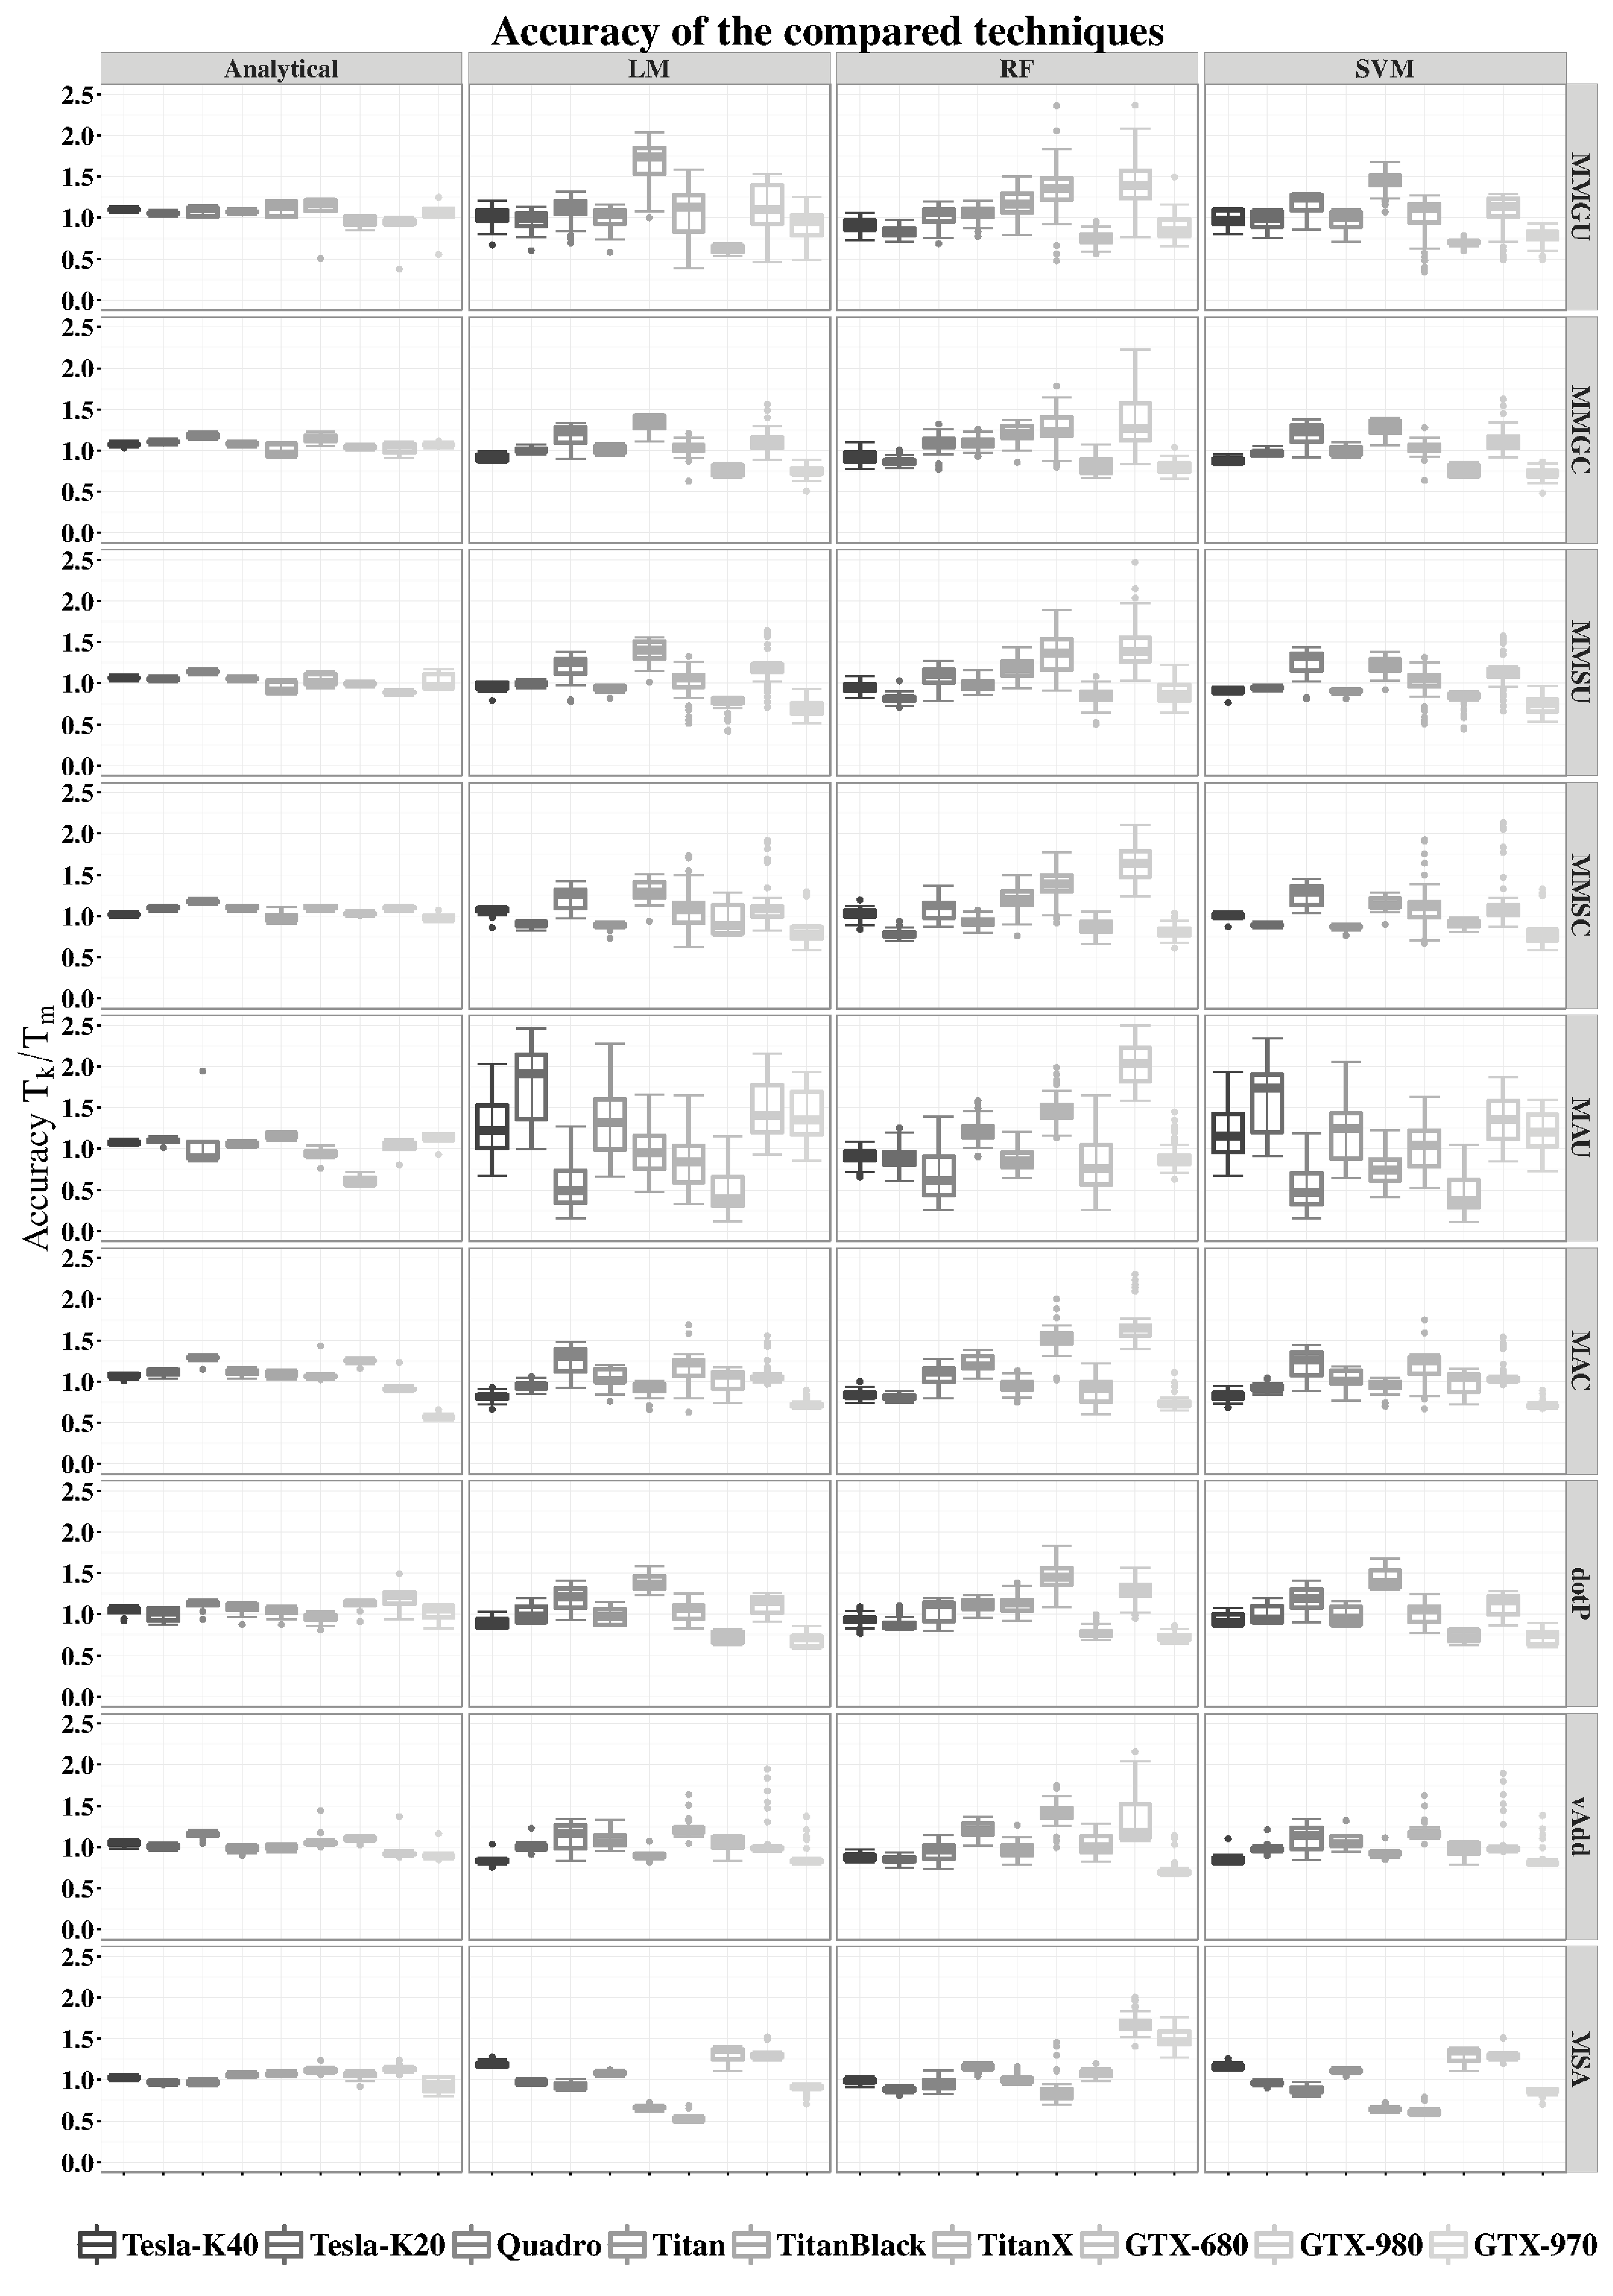
\includegraphics[scale=.3]{./images/ResultTechniques.eps}
 \caption{Accuracy of compared techniques to predict execution times of applications on each GPU.}
 \label{fig:AccuracyAM}
\end{figure*}

Table~\ref{tab:Techniques} shows the comparison between both analytical model and machine learning approaches in terms of normalized mean squared error (MSE). This table shows that although the analytical model obtained the best predictions for almost all the cases, machines  learning  techniques  also provided good predictions. Our next step is to use feature extraction to improve these predictions.

\begin{table}[htpb]
\centering
\caption{Normalized MSE of the different techniques used}
\scalebox{0.7}{
\small
\begin{tabular}{| c | c | c  |  c | c |} 
\midrule%inserts double horizontal lines
\multirow{2}{*}{\textbf{Apps}}&\multicolumn{4}{c|}{\textbf{NMSE}}\\
&\textbf{AM}&\textbf{LR}&\textbf{SVM}&\textbf{RF}\\\midrule
MMGU&\textbf{0.0291}&0.105&0.061&0.096\\
MMGC&\textbf{0.0110}&0.036&0.036&0.079\\
MMSU&\textbf{0.007}&0.055&0.040&0.071\\
MMSC&\textbf{0.008}&0.046&0.044&0.097\\
MAC&\textbf{0.047}&0.293&0.212&0.262\\
MAU&0.044&0.037&\textbf{0.035}&0.114\\
dotP&\textbf{0.015}&0.052&0.054&0.061\\
VecA&\textbf{0.010}&0.021&0.018&0.062\\
MSA&\textbf{0.007}&0.066&0.059&0.087\\   \midrule
\end{tabular}
}
\label{tab:Techniques} 
\end{table}

\section{Conclusions and Future Works}\label{sec:Conclusions}
We performed a fair comparison between analytical model and machine learning techniques to predict the execution times of applications running on GPUs using similar parameters to both approaches. The machine learning techniques were Linear Regression, Support Vector Machine and Random Forest.

The Analytical model provides relatively better prediction accuracy than machine learning approaches, but it requires calculations to be performed for each application. Furthermore, the value of $\lambda$ has to be calculated for each application executing on each GPU.

Machine learning could predict execution time with less accuracy than the analytical model, but this approach provides more flexibility because performing specific calculations is not needed as in the analytical model. A machine learning approach is more generalizable for different applications and GPU architectures than an analytical approach.

As future work, we will consider other irregular benchmarks (Rodinia, Sparse and dense matrix linear algebra operation kernels and graph algorithms). We will also consider the scenario of multiple kernels and GPUs where global synchronization among kernels and one extra memory level, the CPU RAM, needs to be considered.

Also for the learning process in the machine learning: we will perform feature selection from a large set of features (All profiling and metrics data) to choose the most relevant ones and try them on all the regression models we tried before.